\documentclass[10pt,a4paper]{article}
\renewcommand{\baselinestretch}{1.0}
\usepackage{cite}
\usepackage[dvips]{graphicx}
\usepackage{psfrag}
\usepackage{color}
\usepackage[cmex10]{amsmath}
\usepackage{amsfonts}
\usepackage[font=footnotesize, captionskip=10pt]{subfig}
\usepackage{tikz}
\usepackage{flushend}
\usepackage{times}
\usepackage[margin=1.5cm]{geometry}
\usepackage[slovak]{babel}
\usepackage[utf8]{inputenc}
\usepackage[T1]{fontenc}
\usepackage[]{algorithm2e}


\pagestyle{empty}

\hyphenation{net-works}
\newtheorem{remark}{Remark}

\begin{document}

\title{Extrakcia báz rýchlosti z toku červených krviniek ako nástroj na porovnanie modelov}
\author{autor a,b,c,d}
\date{}
\maketitle
\thispagestyle{empty}


\section{Popis problému}

Sú dané kanály mikrofluidného zariadenia A a B (sem by som dal obrázky).
Existujú namerané toky červených krviniek - pre rôzne počty krviniek aj rôzne počiatočné podmienky.
Kedže pri každom nadstavení experimentu sú dráhy rozdielne - v chápani súradníc $(t, x, y, z)$,
nie je možné použiť priame porovnanie.
Je potrebné nájsť invarianty, ktoré by bolo možné porovnať.
Cieľom experimentu je nájsť bázy pre každé meranie a overiť mieru zhody pre kanál A a B.


{\bf Očakávanie} : v rámci spoločného kanála sa očakáva silnejšia korelácia medzi bázami,
predpokladá sa malá závislosť na počiatočných podmienkach aj počtu krviniek. Dominantný
vplyv bude mať tvar kanála.


\subsection{Návrh experimentov}

K dispozícií bolo niekoľko dát zo simulacií tokov. Vstupom do nami navrhovaného experimentu
boli pozície a rychlosti tokov krviniek počas behu simulácie.

Prehľad je znázornený v tabuľke \ref{tab:experiments}.

\begin{table}[ht]
\centering
\caption{Vstupné dáta}
\label{tab:experiments}
\begin{tabular}{|l|l|l|l|}
\hline
experiment & kanál                    & {\color[HTML]{000000} seed} & {\color[HTML]{000000} počet krviniek} \\ \hline
0          & {\color[HTML]{FE0000} A} & {\color[HTML]{000000} a}    & {\color[HTML]{000000} 20}             \\ \hline
1          & {\color[HTML]{FE0000} A} & {\color[HTML]{000000} a}    & {\color[HTML]{000000} 50}             \\ \hline
2          & {\color[HTML]{FE0000} A} & {\color[HTML]{000000} a}    & {\color[HTML]{000000} 100}            \\ \hline
3          & {\color[HTML]{FE0000} A} & {\color[HTML]{000000} b}    & {\color[HTML]{000000} 50}             \\ \hline
4          & {\color[HTML]{FE0000} A} & {\color[HTML]{000000} c}    & {\color[HTML]{000000} 50}             \\ \hline
5          & {\color[HTML]{3531FF} B} & {\color[HTML]{000000} a}    & {\color[HTML]{000000} 50}             \\ \hline
6          & {\color[HTML]{3531FF} B} & {\color[HTML]{000000} b}    & {\color[HTML]{000000} 50}             \\ \hline
\end{tabular}
\end{table}

V prvom priblížení bude model lineárnou kombináciou báz $B_i$,

\begin{align}
 V_j(r) = \sum_{i=1}^{K} w_i(r)V_{B_i}
 \label{eq:lin_model}
\end{align}

kde \\
$K$ je počet bázových funkcií, \\
$B_i$ sú bázy a $V_{B_i}$ predstavuje rýchlostnú zložku bázi, \\
$w_i$ je váha i-tej bázy pre polohu krvinky $r$, \\
$V_j$ je predikovaná rýchlosť j-tej krvinky v polohe $r$, \\


\subsection{Učenie báz}

Zvolený mechanizmus učenia báz je veľmi podobný Kohonenovým sietiam \cite{bib:kohonen_network},
kde sa váhy neurónov upravujú tak aby čo najlepšie pokrili vstupný priestor, k nim
prislúchajú asociačné váhy - požadovaná hodnota výstupu. V uvedenej literatúre
bola Kohonenovám mapa použitá na riešenie úlohy inverznej kinematiky ramena, čo je úloha podobná s problémom nášho
experimentu - hľadá sa asociácia medzi polohou a rýchlosťou v danom bode.

Pre každý experiment sa učenie spustilo nezávisle.
Počiatočné hodnoty báz boli vybrané z náhodne vybraných polôh a rýchlosti krviniek.
Učenie báz prebieha predkladaním polohy krvinky $R_{C}$ a jej rýchlosti $V_{C}$.
Báza má dve zložky polohová $R_{B_i}$, a rýchlostná $V_{B_i}$.
Obe sa upravujú identickými vzťahmi (zodpovedajú metóde stochastic gradient descent \cite{bib:gradient_descent})

\begin{align}
  R_{B_i} &= (1 - \eta\alpha_i)R_{B_i} + \eta\alpha_i R_{C} \\
  V_{B_i} &= (1 - \eta\alpha_i)V_{B_i} + \eta\alpha_i V_{C}
  \label{eq:weight_learn}
\end{align}

parameter $\eta \in (0, 1)$ predstavuje rýchlosť adaptácie báz a $\alpha_i$ je miera podobnosti
polôh $R_{B_i}$ a $R_{C}$. Spočíta sa pomocou podobnostnej funkcie \footnote{môže byť použitá aj iná,
napr. Gaussova - časová zložitosť uvedenej je však menšia}
podľa nasledujúcich vzťahov.



\begin{align}
  \beta_i &=  \frac{k}{k + \left\lVert R_{B_i} - R_{C_i} \right\rVert^2} \label{eq:beta_calc} \\
  \alpha_i &= \frac{\beta_i}{\sum_{j=1}^{K}\beta_j} \label{eq:alpha_calc}
\end{align}

kde parameter $k > 0$ predstavuje strmosť podobnostnej funkcie. Zo vzťahu je zrejmé,
že $\alpha_i \in (0, 1)$, pre blízke polohy je sa hodnota blíži 1, pre vzdialené bunky sa blíži 0.
Druhá rovnica predstavuje normovanie hodnôt $\alpha_i$ tak aby ich súčet bol 1.
Zvolený počet báz bol $K = 10000$, parameter $k = 0.01$ a rýchlosť učenia $\eta = 0.1$. Zvolený počet
iterácií bol $500 000$.



\subsection{Rekonštrukcia polohy a rýchlosti bunky}

Po natrénovaní báz je možné otestovať predikčné schopnosti modelu.
Vstupom je ľubovolná poloha $R_{T}$, cieľom je predpovedať aká bude rýchlosť $V_{T}$ v tomto bode.

Najskôr sa spočítajú honodty $\alpha_i$ podľa vzťahov \ref{eq:beta_calc} a \ref{eq:alpha_calc}, ktoré korešpondujú s váhami $w_i \equiv \alpha_i$.
Pomocou vzťahu \ref{eq:lin_model} sa spočíta rýchlosť v danom bode.

Numerickou integráciou je možné získať trajektóriu testovanej bunky $R_{T}(n+1) = R_{T}(n) + V_{C}(n)dt$.

\section{Výsledky}

Po natrénovaní modelu bolo možné stanoviť rýchlosti v celom priereze kanála -
aj v miestach kde žiadna bunka z trénovacej množiny nešla. Vďaka tomu
bolo možné porovnávať experimenty medzi sebou.

Pre veľký objem dát nie vhodné odčítať všetky body, preto sa metódou Monte Carlo vybralo 1000 náhodných pozícií $R_{T}$.
Výsledná vzdialenosť báz je počítaná normovanou euklidovou metrikou.
Najskôr sa určia rýchlostné zložky báz dvoch natrénovaných modelov $X$, $Y$ pre polohu $R_{T}$.
$V_{xT} = X(R_{T})$ a $V_{yT} = Y(R_{T})$, kde $R_{T}$ predstavuje náhodnú testovaciu polohu.
Rozdiel polôh je spočítaný ako $d_T = \left\lVert V_{xT} - V_{yT} \right\rVert$. Takto vybraných 1000 pozícií
je spriemerovaných. Porovnával sa každý model s každým, výsledky rozdielu sú v tabuľke \ref{tab:model_errors}.

\begin{table}[ht]
\centering
\caption{Veľkosť chyby medzi jednotlivými modelmi}
\label{tab:model_errors}
\begin{tabular}{|l|l|l|l|l|l|l|l|}
\hline
        & model 0                         & model 1                         & model 2                         & model 3                         & model 4                         & model 5                         & model 6                         \\ \hline
model 0 & {\color[HTML]{FE0000} 0}        & {\color[HTML]{FE0000} 0.024045} & {\color[HTML]{FE0000} 0.026852} & {\color[HTML]{FE0000} 0.029994} & {\color[HTML]{FE0000} 0.028294} &  0.069815 &  0.065913 \\ \hline
model 1 & {\color[HTML]{FE0000} 0.024174} & {\color[HTML]{FE0000} 0}        & {\color[HTML]{FE0000} 0.011605} & {\color[HTML]{FE0000} 0.025831} & {\color[HTML]{FE0000} 0.023463} &  0.062432 &  0.064022 \\ \hline
model 2 & {\color[HTML]{FE0000} 0.026618} & {\color[HTML]{FE0000} 0.011235} & {\color[HTML]{FE0000} 0}        & {\color[HTML]{FE0000} 0.027454} & {\color[HTML]{FE0000} 0.026459} &  0.063747 &  0.061519 \\ \hline
model 3 & {\color[HTML]{FE0000} 0.028648} & {\color[HTML]{FE0000} 0.025418} & {\color[HTML]{FE0000} 0.027196} & {\color[HTML]{FE0000} 0}        & {\color[HTML]{FE0000} 0.022168} &  0.064810 &  0.066823 \\ \hline
model 4 & {\color[HTML]{FE0000} 0.026980} & {\color[HTML]{FE0000} 0.026299} & {\color[HTML]{FE0000} 0.026794} & {\color[HTML]{FE0000} 0.022792} & {\color[HTML]{FE0000} 0}        &  0.063020 &  0.062761 \\ \hline
model 5 &  0.066236 &  0.067181 &  0.063129 &  0.067300 &  0.064338 & {\color[HTML]{3531FF} 0} & {\color[HTML]{3531FF} 0.020975} \\ \hline
model 6 &  0.065729 &  0.066606 &  0.062175 &  0.063798 &  0.064817 & {\color[HTML]{3531FF} 0.022061} & {\color[HTML]{3531FF} 0} \\ \hline
\end{tabular}
\end{table}

Experimenty kde sa očakáva menšia chyba (rovnaké kanály) majú spoločnú farbu - červenú pre kanál A a modrú pre kanále B.
Z hodnôt je zrejmé, že modely sa líšia s menšou chybou pre rovnaký kanál. Linearita a jednoduchosť
modelu však spôsobuje aj rozdiely v spoločnom kanály - príčinou sú ako aj rôzne počiatočné podmienky experimentu,
ale aj fakt, že model neuvažuje kolízie buniek a nelinearitu vzťahov.

V ďalšom smerovaní sa treba zamerať na nelineárne modelovanie, napr. pomocou techník deep learning.

Ďalej sme vykonali test kde sa dáta rozdelil na dve časti - trénovaciu a testovaciu (každý experiment nezávisle).
Na testovanie sa zvolilo 25\% dát. Merala sa odchýlka požadovanej rýchlosti od predikovanej rýchlosti modelom.
Výsledky sú uvedené v tabuľke \ref{tab:model_prediction_errors}.



\begin{table}[]
\centering
\caption{chyba predikcie modelov}
\label{tab:model_prediction_errors}
\begin{tabular}{|l|l|l|l|}
\hline
experiment & absolútna chyba & absolútna veľkosť vektora & MRE {[}\%{]} \\ \hline
0          & 0.029266        & 0.253014                  & 11.047184    \\ \hline
1          & 0.037301        & 0.253148                  & 14.865701    \\ \hline
2          & 0.021849        & 0.131263                  & 16.436213    \\ \hline
3          & 0.038164        & 0.259319                  & 14.196479    \\ \hline
4          & 0.040760        & 0.255995                  & 14.843164    \\ \hline
5          & 0.034798        & 0.256949                  & 13.244931    \\ \hline
6          & 0.038682        & 0.246271                  & 15.349910    \\ \hline
\end{tabular}
\end{table}

\subsection{Predikcia tokov pre kanál A}

Model je možné použit na predikciu výsledku experimentu. Zvolili sme experiment 5 na otestovanie tejto hypotézy,
model sme natrénovali pomocou experimentou 0 až 4, všetky pre kanál A, ale rôzne počty krviniek aj seed. Testovalo
sa s inym seed (c). Požadované dráhy sú na obrázku \ref{img:required_trajectory} a dráhy získané z modelu sú na obrázku
\ref{img:resulted_trajectory_all}. Druhý test vznikol trénovaním len na dátach s počtom krviniek 50 - experimenty 1 a 3. Je vidno že model dokáže predpovedať trajektórie. Pre jeho jednoduchosť, však dochádza
aj k chybám - napr. krvinka prechádza cez pevnú prekážku,
alebo nevie zachytit zmenu prúdnice krvinky  (zvíraznené oblasti obrázkov \ref{img:resulted_trajectory_all} a \ref{img:resulted_trajectory}).


\begin{figure}[!ht]
\centering
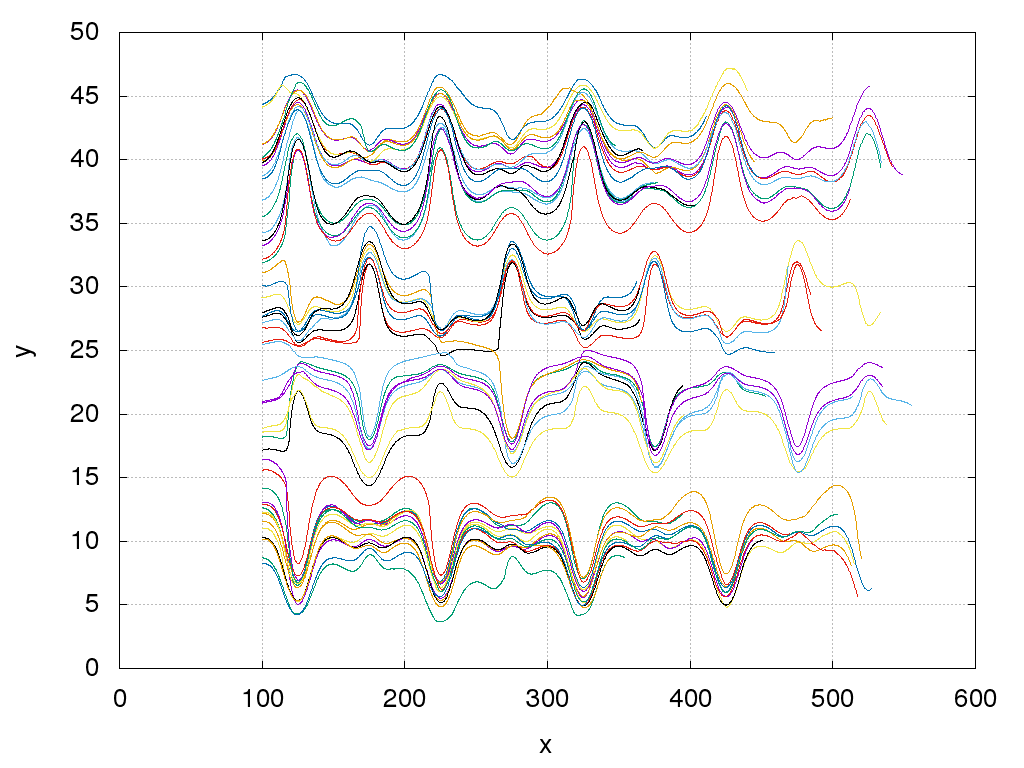
\includegraphics[width=8cm]{images/prediction_required.png}
\caption{požadované trajektórie}
\label{img:required_trajectory}
\end{figure}


\begin{figure}[!ht]
\centering
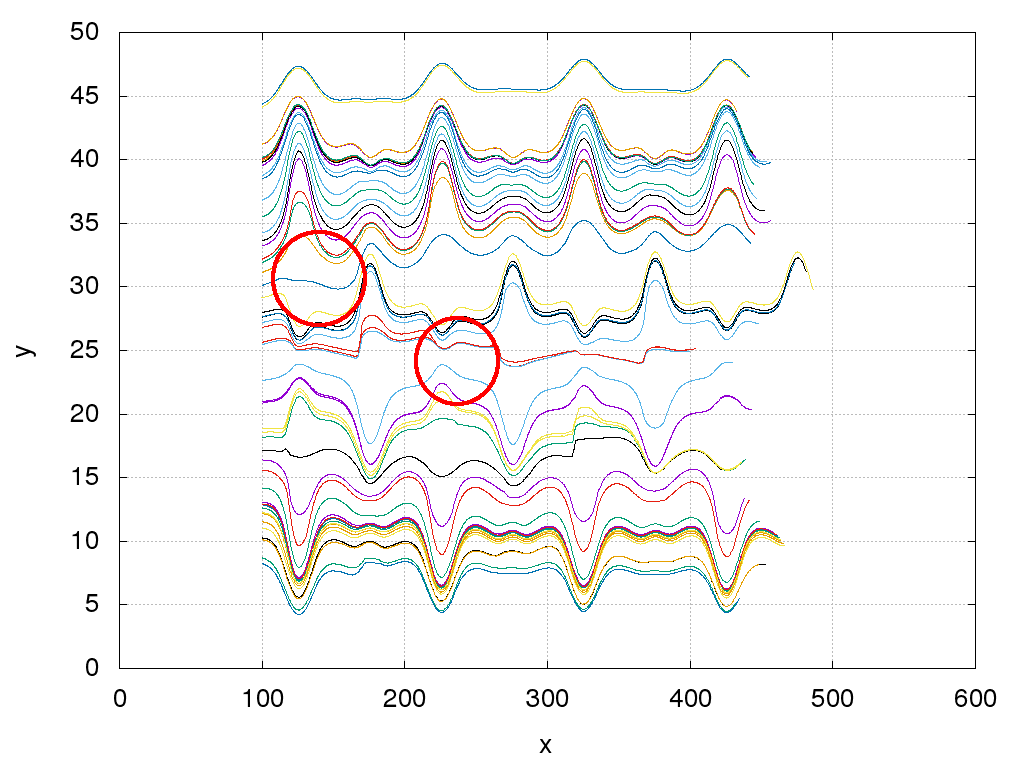
\includegraphics[width=8cm]{images/prediction_resulted_errors.png}
\caption{získané trajektórie trénované na všetkych dátach}
\label{img:resulted_trajectory_all}
\end{figure}


\begin{figure}[!ht]
\centering
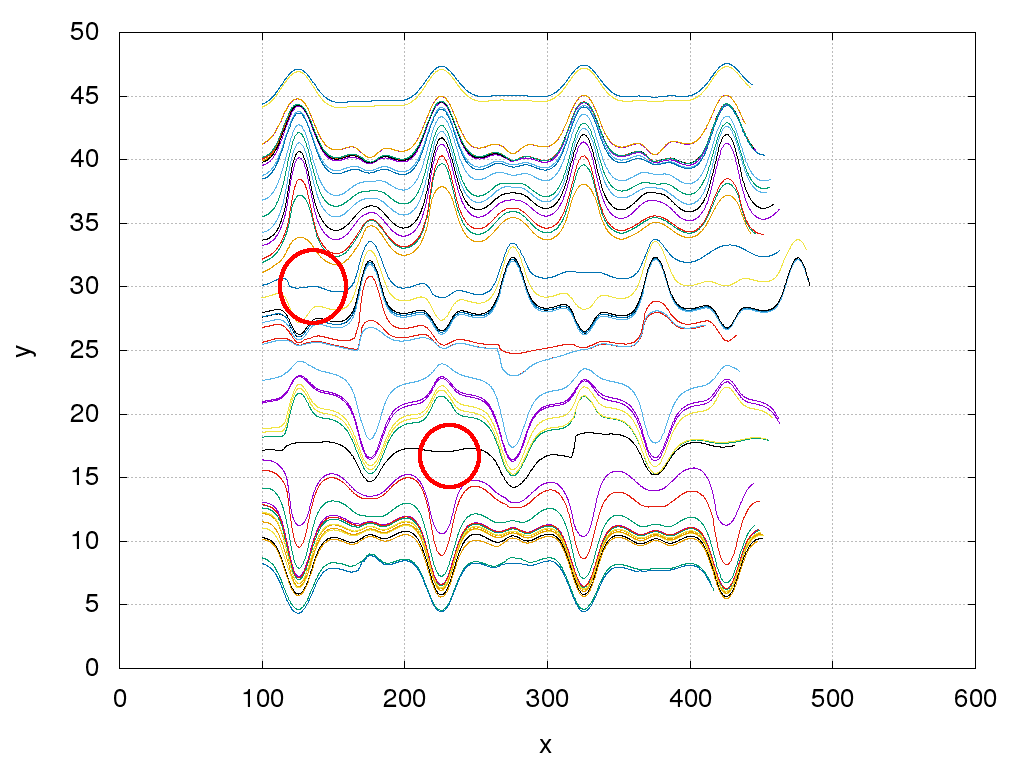
\includegraphics[width=8cm]{images/prediction_resulted_50_errors.png}
\caption{získané trajektórie trénované len na dátach experimentu 1 a 3}
\label{img:resulted_trajectory}
\end{figure}




\subsection{Aproximácia tokov pre kanál A}

Nasledujúce obrázky predstavujú rýchlosti buniek $\left\lVert V_{C} \right\rVert$ v celom priereze kanála A tak ako boli
získané z trénovania experimentov 0 až 4.

\begin{figure}[!ht]
\centering
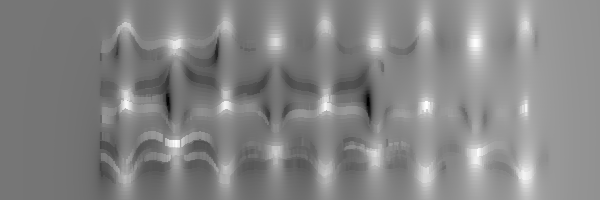
\includegraphics[width=8cm]{images/e0_approximation_size.png}
\caption{experiment 0}
\label{img:experiment0}
\end{figure}

\begin{figure}[!ht]
\centering
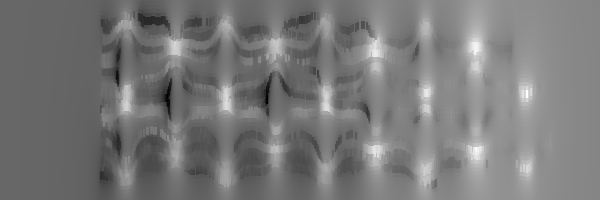
\includegraphics[width=8cm]{images/e1_approximation_size.png}
\caption{experiment 1}
\label{img:experiment1}
\end{figure}

\begin{figure}[!ht]
\centering
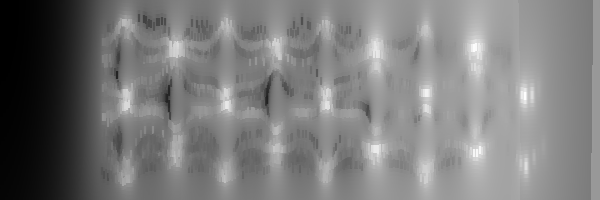
\includegraphics[width=8cm]{images/e2_approximation_size.png}
\caption{experiment 2}
\label{img:experiment2}
\end{figure}

\begin{figure}[!ht]
\centering
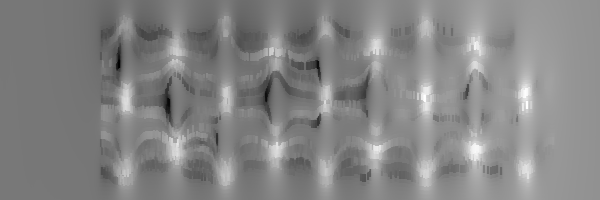
\includegraphics[width=8cm]{images/e3_approximation_size.png}
\caption{experiment 3}
\label{img:experiment3}
\end{figure}


\begin{figure}[!ht]
\centering
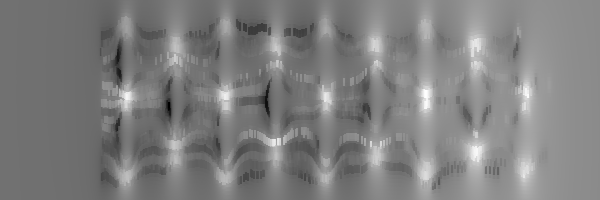
\includegraphics[width=8cm]{images/e4_approximation_size.png}
\caption{experiment 4}
\label{img:experiment4}
\end{figure}

\subsection{Aproximácia tokov pre kanál B}

Nasledujúce obrázky predstavujú rýchlosti buniek $\left\lVert V_{C} \right\rVert$ v celom priereze kanála B tak ako boli
získané z trénovania experimentov 5 až 6. Model umožňuje získať rýchlosť v ľubovolnom bode.

\begin{figure}[!ht]
\centering
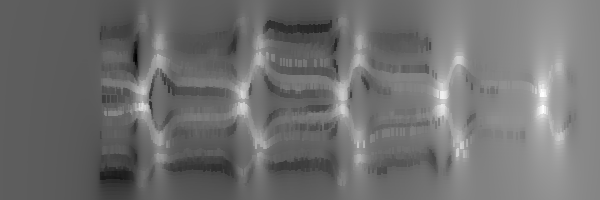
\includegraphics[width=8cm]{images/e5_approximation_size.png}
\caption{experiment 5}
\label{img:experiment5}
\end{figure}

\begin{figure}[!ht]
\centering
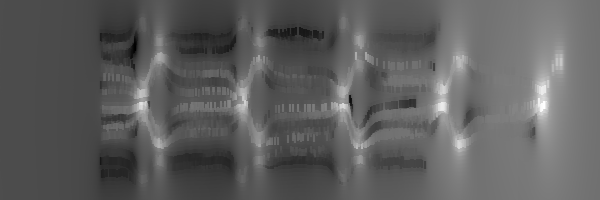
\includegraphics[width=8cm]{images/e6_approximation_size.png}
\caption{experiment 6}
\label{img:experiment6}
\end{figure}


\begin{thebibliography}{9}
\bibitem{bib:kohonen_network}
R. Rojas: Neural Networks, Springer-Verlag, Berlin, 1996, Kohonen Networks

\bibitem{bib:gradient_descent}
Sebastian Ruder, An overview of gradient descent optimization algorithms
\end{thebibliography}




\end{document}
